    \p 
یک مستطیل را با تعدادی مستطیل کوچک‌تر پوشانده‌ایم به‌گونه‌ای که مستطیل‌ها فقط می‌توانند در رئوس و اضلاع با یکدیگر مشترک هستند. همچنین اضلاع مستطیل‌های پوشاننده، موازی اضلاع مستطیل اصلی هستند و هیچ قسمتی از این مستطیل‌ها بیرون از مستطیل اصلی قرار نمی‌گیرند. ثابت کنید مجموع تعداد خطوط افقی، تعداد خطوط عمودی و تعداد چهارراه‌ها برابر با تعداد مستطیل‌های پوشاننده به علاوه‌ی سه است. مثلا در شکل زیر تعداد خطوط عمودی برابر
$5$
، تعداد خطوط افقی برابر
$5$
، تعداد چهارراه‌ها برابر
$2$
و تعداد مستطیل‌های پوشاننده برابر
$9$
است. همچنین
$AB$
یک خط افقی،
$C$
یک چهارراه و
$DEFG$
یک مستطیل پوشاننده است.
\begin{center}
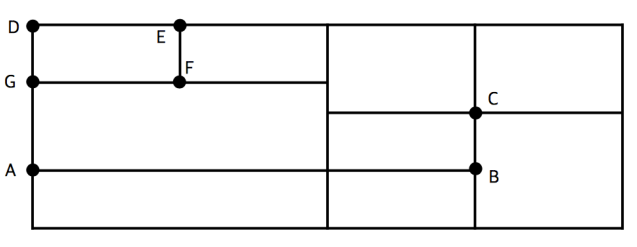
\includegraphics[height=3cm]{1.png}
\end{center}